% Generated by GenerateTaFamilyComparison — do not edit by hand.
% Trilinear-aggregation family: normalised leading constant 3*R(N)/N^3 vs N.
\begin{figure}[t]
  \centering
  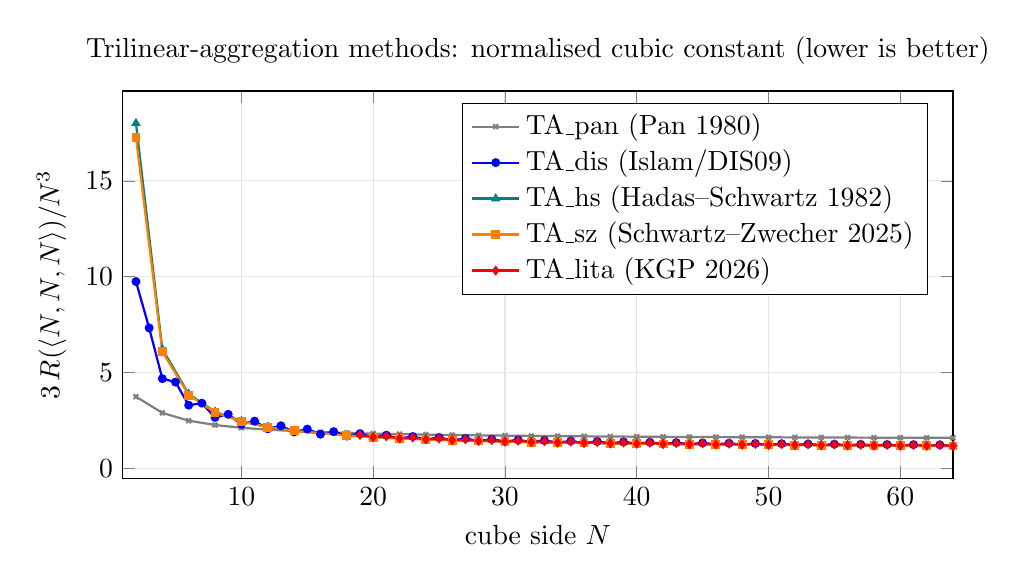
\begin{tikzpicture}
    \begin{axis}[
        width=\linewidth, height=6.5cm,
        xlabel={cube side $N$}, ylabel={$3\,R(\langle N,N,N\rangle)/N^3$},
        xmin=1, xmax=64,
        legend pos=north east, legend cell align=left,
        grid=both, major grid style={black!10}, minor grid style={black!5},
        title={Trilinear-aggregation methods: normalised cubic constant (lower is better)}]
      \addplot[gray, mark=x, mark size=1.2pt, thick] coordinates {(2,3.7500) (4,2.9063) (6,2.5000) (8,2.2734) (10,2.1300) (12,2.0313) (14,1.9592) (16,1.9043) (18,1.8611) (20,1.8263) (22,1.7975) (24,1.7734) (26,1.7530) (28,1.7353) (30,1.7200) (32,1.7065) (34,1.6946) (36,1.6840) (38,1.6745) (40,1.6659) (42,1.6582) (44,1.6511) (46,1.6446) (48,1.6387) (50,1.6332) (52,1.6281) (54,1.6235) (56,1.6191) (58,1.6150) (60,1.6113) (62,1.6077) (64,1.6044)};
      \addlegendentry{TA\_pan (Pan 1980)}
      \addplot[blue, mark=*, mark size=1.2pt, thick] coordinates {(2,9.7500) (3,7.3333) (4,4.6875) (5,4.5120) (6,3.3056) (7,3.4111) (8,2.6719) (9,2.8313) (10,2.3100) (11,2.4748) (12,2.0764) (13,2.2340) (14,1.9133) (15,2.0604) (16,1.7930) (17,1.9296) (18,1.7006) (19,1.8274) (20,1.6275) (21,1.7454) (22,1.5682) (23,1.6781) (24,1.5191) (25,1.6220) (26,1.4778) (27,1.5745) (28,1.4426) (29,1.5336) (30,1.4122) (31,1.4982) (32,1.3857) (33,1.4672) (34,1.3625) (35,1.4399) (36,1.3418) (37,1.4155) (38,1.3234) (39,1.3937) (40,1.3069) (41,1.3741) (42,1.2920) (43,1.3563) (44,1.2784) (45,1.3402) (46,1.2661) (47,1.3254) (48,1.2548) (49,1.3119) (50,1.2444) (51,1.2995) (52,1.2348) (53,1.2880) (54,1.2260) (55,1.2773) (56,1.2178) (57,1.2674) (58,1.2102) (59,1.2582) (60,1.2031) (61,1.2496) (62,1.1964) (63,1.2416) (64,1.1902)};
      \addlegendentry{TA\_dis (Islam/DIS09)}
      \addplot[teal, mark=triangle*, mark size=1.2pt, thick] coordinates {(2,18.0000) (4,6.2344) (6,3.8889) (8,2.9590) (10,2.4720) (12,2.1753) (14,1.9767) (18,1.7284) (20,1.6459) (22,1.5800) (24,1.5263) (26,1.4816) (28,1.4438) (30,1.4116) (32,1.3836) (34,1.3593) (36,1.3378) (38,1.3187) (40,1.3017) (42,1.2864) (44,1.2725) (46,1.2600) (48,1.2485) (50,1.2380) (52,1.2284) (54,1.2195) (56,1.2113) (58,1.2036) (60,1.1965) (62,1.1899) (64,1.1837)};
      \addlegendentry{TA\_hs (Hadas--Schwartz 1982)}
      \addplot[orange, mark=square*, mark size=1.2pt, thick] coordinates {(2,17.2500) (4,6.0938) (6,3.8333) (8,2.9297) (10,2.4540) (12,2.1632) (14,1.9679) (18,1.7233) (20,1.6418) (22,1.5766) (24,1.5234) (26,1.4792) (28,1.4418) (30,1.4098) (32,1.3821) (34,1.3579) (36,1.3365) (38,1.3176) (40,1.3007) (42,1.2855) (44,1.2717) (46,1.2592) (48,1.2478) (50,1.2374) (52,1.2278) (54,1.2189) (56,1.2108) (58,1.2032) (60,1.1961) (62,1.1895) (64,1.1833)};
      \addlegendentry{TA\_sz (Schwartz--Zwecher 2025)}
      \addplot[red, mark=diamond*, mark size=1.2pt, thick] coordinates {(19,1.7565) (20,1.6376) (21,1.6838) (22,1.5733) (23,1.6239) (24,1.5206) (25,1.5736) (26,1.4768) (27,1.5310) (28,1.4397) (29,1.4942) (30,1.4080) (31,1.4621) (32,1.3805) (33,1.4339) (34,1.3565) (35,1.4091) (36,1.3353) (37,1.3868) (38,1.3165) (39,1.3669) (40,1.2997) (41,1.3489) (42,1.2846) (43,1.3327) (44,1.2709) (45,1.3178) (46,1.2585) (47,1.3042) (48,1.2472) (49,1.2918) (50,1.2368) (51,1.2803) (52,1.2272) (53,1.2697) (54,1.2184) (55,1.2599) (56,1.2103) (57,1.2507) (58,1.2027) (59,1.2422) (60,1.1957) (61,1.2342) (62,1.1891) (63,1.2268) (64,1.1829)};
      \addlegendentry{TA\_lita (KGP 2026)}
    \end{axis}
  \end{tikzpicture}
  \caption{Each trilinear-aggregation method gives an alternative rank for $\langle N,N,N\rangle$ over its own domain (TA\_pan/TA\_hs/TA\_sz are even only, TA\_hs/TA\_sz exclude the $N{=}16$ pole, TA\_lita requires $N\ge 19$). Plotted is the normalised leading constant $3R/N^3$; all converge to $1$, and the crossovers show which method is tightest over which range --- TA\_lita (KGP 2026) dominates for odd $N\ge 19$ and large even $N$, while TA\_dis still wins at e.g.\ $N{=}22$.}
  \label{fig:ta-family-ranks}
\end{figure}
